\chapter{Background}

\section{Model Checking}
During the course of this project, I have familiarized myself with the concept of model checking.~\cite{modelChecking}
Formal software verification uses mathematically precise proofs to verify the correctness of computer programs. Model checking is a widely used method that exhaustively checks every possible execution of a program for every possible input to see if certain properties are satisfied.
In my case, I focused mainly on reachability testing, which means we explore the state space of a program to see if a certain bad state can be reached.

\begin{figure}[h]
  \centering
  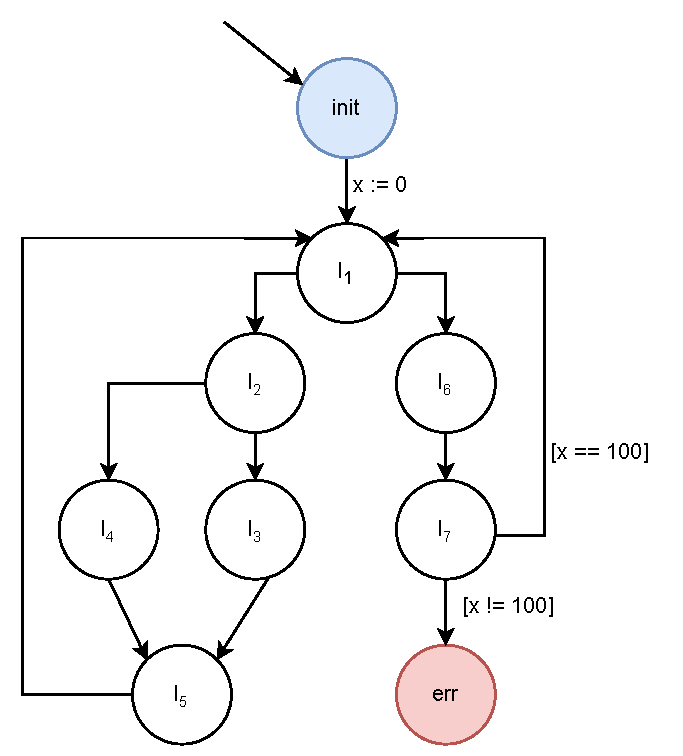
\includegraphics[width=0.5\textwidth]{figures/cfa_simple.pdf}
  \caption{Simple representation of a Control-Flow Automata (CFA).}
  \label{fig:cfa}
\end{figure}

To perform model checking, we first need to represent the program in a way that makes its control and data flow analyzable. This is where the concept of a \textbf{Control-Flow Automaton (CFA)} becomes useful. Figure~\ref{fig:cfa} illustrates a simplified CFA, which models how control moves between different parts of a program.

A CFA consists of:
\begin{itemize}
  \item \textbf{Locations} — These represent program points (e.g., line numbers or steps) and are shown as circles in the figure. The blue circle denotes the \textit{initial state}, and the red circle marks the \textit{error state}.
  \item \textbf{Edges} — These indicate transitions between locations and represent operations such as assignments or conditional checks. In the figure, they are visualized as arrows.
\end{itemize}

It helps in analyzing programs, especially for checking if errors (like reaching a bad state) can happen.~\cite{cfa}. In this documentation, I will describe how a BTOR2 program can be transformed into a CFA, and how this representation supports effective model checking.


\section{BTOR2}
% BTOR2C tool mire jó 
The Hardware Model Checking Competition (HWMCC)\footnote{\url{https://hwmcc.github.io/}} serves as a benchmark for evaluating formal verification tools for hardware systems. A key innovation supporting this effort is BTOR2, a word-level model checking format designed for bit-precise modeling. Building on the earlier BTOR format, BTOR2~\cite{btor2} introduces a simple, sorted, line-based syntax that is easy to parse and aligns with SMT-LIB semantics for bit-vectors and arrays.~\cite{SMT-LIB} It combines the low-level precision of formats like AIGER with higher-level abstractions, making it ideal for various verification techniques.~\cite{AIGER}

\begin{figure}[h]
  \centering
  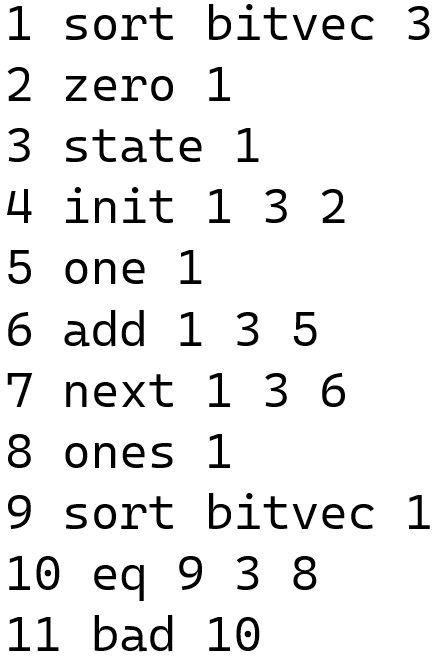
\includegraphics[width=0.2\textwidth]{figures/count2.png}
  \caption{ Syntax of Btor2. count2.btor2 example. }
  \label{fig:count2}
\end{figure}

In Figure~\ref{fig:count2} is a BTOR2 circuit that defines a simple finite state machine — a 3-bit counter — that starts from zero and increments by one at each time step. The specification is written in the BTOR2 format, which is a line-based syntax used to describe word-level sequential circuits. Each line defines a node in the circuit, such as a constant, state, operation, or property.

At the beginning of the circuit, line 1 declares a bit-vector sort of width 3 \verb|sort bitvec 3|, which serves as the type for all 3-bit values used throughout the circuit. Line 2 defines a constant zero \verb|zero 1|, which produces the bit-vector \verb|000|. Following this, line 3 introduces a state variable of sort 1 (3 bits), representing the main state of the circuit.

The initial value of this state is specified in line 4, which uses the init keyword to bind state 3 to start at constant 2, which is the \verb|000| bit-vector. The next input is defined in line 5 using one 1, which denotes the constant \verb|001|.

Line 6 defines an addition operation that adds the current state value (3) with 1, resulting in node 6, the next value of the counter. This operation wraps around on overflow due to the fixed 3-bit width. Line 7 then uses the next keyword to specify that in the next state, the counter should take the value of node 6, i.e., the incremented result.

To define a property of interest, line 8 declares another constant: \verb|ones 1|, which represents the maximum value a 3-bit counter can hold—namely \verb|111|. Line 9 introduces a new sort of width 1, which is used for boolean-like signals such as equality checks.

Line 10 defines a comparison between the current counter value and the maximum value \verb|111| using the eq operator. This operation returns a 1-bit result: true (1) if the counter is at maximum, false (0) otherwise. Finally, line 11 marks this equality result as a bad state, which is a property violation. Hence, the circuit asserts that reaching the value 111 is undesirable or erroneous.

In summary, this BTOR2 circuit models a 3-bit counter that increments with each step and triggers a bad state when it reaches 111. This design could be used in formal verification to prove that the system avoids overflow, or alternatively, to find the point at which it does. The clear structure and modular nature of BTOR2 make it suitable for such sequential hardware modeling and property checking.

Btor2C is a tool that translates Btor2 hardware models into equivalent C programs. This allows software verification tools to analyze hardware designs, bridging the gap between hardware and software verification. ~\cite{btor2c}
In my implementation, I focused on bit-vectors and their related functions and definitions, leveraging the expressive power of BTOR2 to model and verify small, bit-precise sequential systems.

\section{ANTLR}
We have written an unofficial BTOR2 grammar format using ANTLR4~\cite{antlr}.
ANTLR (ANother Tool for Language Recognition) is a powerful parser generator widely used in both academia and industry to build interpreters, compilers, and DSLs. Based on LL parsing, it reads grammar files and automatically generates lexers and parsers for multiple languages, including Java, C++, and Python. ANTLR cleanly separates syntax from application logic using \textit{listener} and \textit{visitor} patterns, enabling maintainable and modular code.
This makes ANTLR an excellent tool for writing a BTOR2 grammar, as its clear structure, support for complex syntax rules, and language flexibility make it easy to build robust parsers for BTOR2's line-based, sorted format.

\section{Theta}
My main goal was to achieve a BTOR2 frontend for the Theta model checker.\cite{theta}
Theta is a modular and extensible model checking framework developed by the Critical Systems Research Group at the Budapest University of Technology and Economics. It is designed to support a wide range of verification techniques, particularly abstraction refinement-based reachability analysis, and is capable of analyzing various low-level formalisms such as Control Flow Automata (CFA), Symbolic Transition Systems (STS), and Timed Automata.
One of Theta's major strengths is its support for high-level frontends, allowing users to model complex systems in languages like C or statecharts, which are then automatically translated into formal representations. This makes Theta highly accessible and adaptable for both research and practical applications.
In my project, I used XCFA models, an extension of CFA that includes support for procedures and concurrency, but I focused specifically on the CFA parts, applying Theta's powerful CEGAR-based algorithms for reachability checking.